\subsection{Indefinite Integrals}\label{subsec-indefinite-integrals}


\begin{definition}\label{def-indefinite-integral}
	The anti-derivative $F$ of a function $f$ on $I$ is defined such that
	\begin{equation}
		\forall x\in I:  F'(x) = f(x)
	\end{equation}
	When $F$ is an score of anti-derivative of $f$ we denote it by
	\begin{equation}\label{eq-indefinite-integral}
		\int f(x) \diff x = F(x) + C \qquad(C\in\mathbb{R})
	\end{equation}
	where the left-hand side of this equation describes an indefinite integral.
\end{definition}

\begin{exm}\label{exm-indefinite-integral:1}
	Find the indefinite integral of $\sin(x)$ with respect to $x$.
	\begin{flushleft}
		\textbf{Answer}: We can solve the immediate integral using the knowledge
		we obtained during our time when we studied derivatives of functions,
		\textit{i.e.}
		\begin{equation*}
			\int \sin(x) \diff x = -\cos(x) + C
		\end{equation*}
	\end{flushleft}
\end{exm}

\begin{exm}\label{exm-indefinite-integral:2}
	Find the indefinite integral of $x$ with respect to $x$.
	\begin{flushleft}
		\textbf{Answer}:
		\begin{equation*}
			\int x \diff x = -\frac{1}{2}x^2 + C
		\end{equation*}
	\end{flushleft}
\end{exm}

\begin{thm}\label{thm-indefinite-integral-linearity}
	Let $f$ and $g$ be two integrable functions, and let $\lambda\in\mathbb{R}$.
	Then indefinite integral satisfy the linearity property:
	\begin{enumerate}
		\item Addition:
		      \begin{equation}\label{eq-indefinite-integral-linearity:1}
			      \int \left(f(x)+g(x)\right) \diff x = \int f(x) \diff x + \int g(x) \diff x
		      \end{equation}
		\item Multiplication with a scalar:
		      \begin{equation}\label{eq-indefinite-integral-linearity:2}
			      \int \left(\lambda f(x)\right) \diff x = \lambda \int f(x) \diff x
		      \end{equation}
	\end{enumerate}
\end{thm}

\begin{exm}\label{exm-indefinite-integral:3}
	Find the indefinite integral of $\tfrac{x^4}{1+x^2}$ with respect to $x$.
	\begin{flushleft}
		\textbf{Answer}:
		\begin{align*}
			\int \frac{x^4}{1+x^2} \diff x & = \int \frac{x^4-1+1}{1+x^2} \diff x                                                                                \\
			                               & = \int \frac{(x^2-1)(x^2+1)+1}{1+x^2} \diff x                                                                       \\
			                               & = \int (x^2-1) \diff x + \int \frac{1}{1+x^2} \diff x &  & \text{\pref{theorem}{thm-indefinite-integral-linearity}} \\
			                               & = \frac{1}{3}x^3 - x + \arctan(x) + C
		\end{align*}
	\end{flushleft}
\end{exm}

\begin{exm}\label{exm-indefinite-integral:4}
	Find the indefinite integral of $\tan(x)$ with respect to $x$.
	\begin{flushleft}
		\textbf{Answer}: Note, that in general we have that
		\begin{equation}\label{eq-useful-integral}
			\int \frac{f'(x)}{f(x)} \diff x = \ln(\abs{f(x)}) + C \qquad(C\in\mathbb{R})
		\end{equation}
		which can be easily verified by taking the derivative on the right-hand side. Therefore,
		\begin{align*}
			\int \tan(x) \diff x & = \int \frac{\sin(x)}{\cos(x)} \diff x \\
			                     & = -\ln(\abs{\cos(x)}) + C
		\end{align*}
	\end{flushleft}
\end{exm}

\subsubsection{Integration by Parts}\label{subsubsec-integration-by-parts}

\begin{definition}\label{def-integration-by-parts}
	Using integration by parts we can integrate the product of two functions
	$u$,$v$ with respect to $x$ such that
	\begin{align*}
		\underbrace{\int \left(u(x)v(x)\right)' \diff x}_{u(x)v(x)} & = \int u'(x)v(x) \diff x + \int v'(x)u(x) \diff x &  & \text{\pref{definition}{thm-derivative-arithmetic}} \\
		\implies \int v'(x)u(x) \diff x                             & = u(x)v(x) - \int u'(x)v(x) \diff x
	\end{align*}
\end{definition}

\begin{exm}\label{exm-integration-by-parts:1}
	Use integration by parts to find the indefinite integral of $x\exp(x)$ with respect to $x$.
	\begin{flushleft}
		\textbf{Answer}: Let $u(x)=x$ and $v'(x)=\exp(x)$. Then,
		$u'(x)=1$ and $v(x)=\exp(x)$, thus
		\begin{align*}
			\int x\exp(x) \diff x & = x\exp(x) - \int 1\exp(x) \diff x \\
			                      & = \exp(x)\left(x-1\right) + C
		\end{align*}
	\end{flushleft}
\end{exm}

\begin{exm}\label{exm-integration-by-parts:2}
	Use integration by parts to find the indefinite integral of $\exp(x)\cos(x)$ with respect to $x$.
	\begin{flushleft}
		\textbf{Answer}: Let $u(x)=\cos(x)$ and $v'(x)=\exp(x)$. Then,
		$u'(x)=-\sin(x)$ and $v(x)=\exp(x)$, thus
		\begin{align*}
			\int \exp(x)\cos(x) \diff x           & = \exp(x)\cos(x) + \int \exp(x)\sin(x) \diff x                               \\
			                                      & = \exp(x)\cos(x) + \left(\exp(x)\sin(x) - \int \exp(x)\cos(x) \diff x\right) \\
			\implies 2\int \exp(x)\cos(x) \diff x & = \exp(x)\cos(x) + \exp(x)\sin(x) + C                                        \\
			                                      & = \frac{\exp(x)}{2}\big(\cos(x)+\sin(x)\big) + C
		\end{align*}
	\end{flushleft}
\end{exm}

\begin{exm}\label{exm-integration-by-parts:3}
	Use integration by parts to find the indefinite integral of $\arctan(x)$ with respect to $x$.
	\begin{flushleft}
		\textbf{Answer}: Note that $\arctan(x)=1\cdot\arctan(x)$. So, let
		$u(x)=\arctan(x)$ and $v'(x)=1$. Then, $u'(x)=\frac{1}{1+x^2}$ and $v(x)=x$, thus
		\begin{align*}
			\int \arctan(x) \diff x & = x\arctan(x) - \int \frac{x}{1+x^2} \diff x                                                    \\
			                        & = x\arctan(x) - \frac{1}{2}\ln(\abs{1+x^2}) + C &  & \text{\pref{equation}{eq-useful-integral}}
		\end{align*}
	\end{flushleft}
\end{exm}

\begin{exm}\label{exm-integration-by-parts:4}
	Find the indefinite integral of $\exp(-\abs{x})$ with respect to $x$.
	\begin{flushleft}
		\textbf{Answer}:
		\begin{align*}
			\int \exp(-\abs{x}) \diff x & = \begin{cases}
				\int \exp(-x) \diff x \text{ if } x\geq0 \\
				\int \exp(x) \diff x \text{ if } x<0     \\
			\end{cases}                    \\
			                            & \overset{(\star)}{=} \begin{cases}
				-\exp(-x) + 2 + C \text{ if } x\geq0 \\
				\exp(x) + C \text{ if } x<0
			\end{cases}
		\end{align*}
	\end{flushleft}
	Notice that we have to fix the discontinuity in $(\star)$ by adding $2$; see
	also \pref{figure}{sketch:exm-integration-by-parts:4}.
	\begin{equation*}
		\exp(-0)+C_1 = \exp(0) + C_2  \implies C_1 = 2 + C_2
	\end{equation*}
	If it weren't for this
	change the function would no longer be continuous (and by extension differentiable
	at $x=0$, \textit{cf.} \pref{remark}{rem-continuity-doesnt-imply-differentiability}),
	which in turn would violate \pref{definition}{def-indefinite-integral}.
	\begin{flushleft}
		\textbf{Left-hand side limit at $x=0$}:
		\begin{align*}
			F_-'(x_0) & = \lim_{h\to0^+}\frac{F(x_0+h)-F(x_0)}{h}                                                              \\
			          & = \lim_{h\to0^+}\frac{\exp(x_0+h)+C-(-\exp(-x_0)+2+C)}{h}                                              \\
			          & = \lim_{h\to0^+}\frac{\exp(x_0)\exp(h)+\exp(x_0)-2}{h}    &  & x_0 = 0                                 \\
			          & = \lim_{h\to0^+}\frac{\exp(h)-1}{h}                       &  & \text{\pref{definition}{def-euler-alt}} \\
			          & = 1
		\end{align*}
		\textbf{Right-hand side limit at $x=0$}:
		\begin{align*}
			F_+'(x_0) & = \lim_{h\to0^-}\frac{F(x_0+h)-F(x_0)}{h}                                                                 \\
			          & = \lim_{h\to0^-}\frac{\exp(-x_0-h)+2+C-(-\exp(-x_0)+2+C)}{h} &  & x_0 = 0                                 \\
			          & = \lim_{h\to0^-}\frac{-\exp(h)+1}{h}                         &  & \text{\pref{definition}{def-euler-alt}} \\
			          & = 1
		\end{align*}
	\end{flushleft}
	\begin{figure}[ht!]
		\centering
		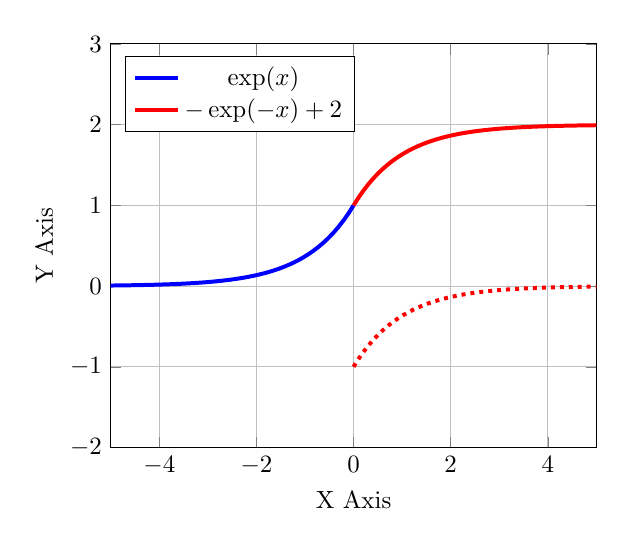
\begin{tikzpicture}[scale=0.9]
			\begin{axis}[
					xmax=5,
					xmin=-5,
					ymax=3,
					ymin=-2,
					samples=50,
					grid=major,
					xlabel={X Axis},
					ylabel={Y Axis},
					legend pos=north west
				]
				\addplot[blue,ultra thick,domain=-5:0]{exp(x)};
				\addplot[red,ultra thick,domain=0:5]{-exp(-x)+2};
				\addplot[red,ultra thick,dotted,domain=0:5]{-exp(-x)};
				\legend{$\exp(x)$,$-\exp(-x)+2$}
			\end{axis}
		\end{tikzpicture}
		\caption{Plot of the indefinite integral of $\exp(-\abs{x})$}
		\label{sketch:exm-integration-by-parts:4}
	\end{figure}
\end{exm}

\subsubsection{Integration of Rational Functions}\label{subsubsec-integration-rational-functions}

\begin{flushleft}
	Rational functions are of the form $\tfrac{p(x)}{q(x)}$ (where $p(x)$ and $q(x)$
	are polynomials and $q(x)\neq0$) that require different approaches when it
	comes to integration depending on the situation at hand. In this subsection
	we will walk through each case step by step by example, rather than proving
	the theorem that provides the underlying theory.
\end{flushleft}

\begin{exm}\label{exm-integration-rational-function:1}
	Find the indefinite integral of
	\begin{equation*}
		\int \frac{2x^4-x^3-x^2+3x-4}{x^2+1} \diff x
	\end{equation*}
	\begin{flushleft}
		\textbf{Answer}: In this example we have to first simplify the expression
		algebraically by performing a long division with polynomials\footnote{See
			also: \url{https://en.wikipedia.org/wiki/Polynomial_long_division}}, the
		result of which is
		\begin{align*}
			\int \frac{2x^4-x^3-x^2+3x-4}{x^2+1} \diff x
			 & = \int \left(2x^2-x-3+\frac{4x-1}{x^2-1}\right) \diff x                                                                                       \\
			 & = \frac{2}{3}x^3 -\frac{1}{2}x^2-3x + \int \frac{4x-1}{x^2-1} \diff x         &  & \text{\pref{example}{exm-integration-rational-function:4}} \\
			 & = \frac{2}{3}x^3 -\frac{1}{2}x^2-3x + \ln(\abs{3x-1}) + \frac{2}{3(3x-1)} + C
		\end{align*}
		\textit{This kind of situation occurs when $\deg(p)>\deg(q)$.}
	\end{flushleft}
\end{exm}

\begin{exm}\label{exm-integration-rational-function:2}
	Find the indefinite integral of
	\begin{equation*}
		\int \frac{1}{2x^2+9x-5} \diff x
	\end{equation*}
	\begin{flushleft}
		\textbf{Answer}: In this example we use \gls{pfd} to split up the integral
		into two parts\footnote{See also: \url{https://en.wikipedia.org/wiki/Partial_fraction_decomposition}}
		\begin{align*}
			\int \frac{1}{2x^2+9x-5} \diff x
			 & = \int \frac{1}{(2x-1)(x+5)} \diff x                                                                                              \\
			 & = \int \frac{A}{2x-1} \diff x + \int \frac{B}{x+5} \diff x                                                                        \\
			 & = \int \frac{\frac{2}{11}}{2x-1} \diff x + \int \frac{-\frac{1}{11}}{x+5} \diff x                                                 \\
			 & = \frac{1}{11}\int \frac{2}{2x-1} - \frac{1}{11} \int \frac{1}{x+5} \diff x       &  & \text{\pref{equation}{eq-useful-integral}} \\
			 & = \frac{1}{11}\ln(\abs{2x-1}) - \frac{1}{11}\ln(\abs{x+5}) + C
		\end{align*}
		\textit{This kind of situation occurs when the denominator $q$ has distinct
			linear factors.}
	\end{flushleft}
\end{exm}

\begin{exm}\label{exm-integration-rational-function:3}
	Find the indefinite integral of
	\begin{equation*}
		\int \frac{9x-5}{9x^2-6x+1} \diff x
	\end{equation*}
	\begin{flushleft}
		\textbf{Answer}: This type of integral is similar to the one we encountered
		in \pref{example}{exm-integration-rational-function:1}, but it has a little
		twist to it as can be observed in the solution below:
		\begin{align*}
			\int \frac{9x-5}{9x^2-6x+1} \diff x
			 & = \int \frac{9x-5}{(3x-1)^2} \diff x                                                                            \\
			 & = \int \frac{A}{3x-1} \diff x + \int \frac{B}{(3x-1)^2} \diff x                                                 \\
			 & = \int \frac{3}{3x-1} \diff x - \int \frac{2}{(3x-1)^2} \diff x &  & \text{\pref{equation}{eq-useful-integral}} \\
			 & = \ln(\abs{3x-1}) + \frac{2}{3}\cdot\frac{1}{3x-1} + C
		\end{align*}
		\textit{This kind of situation occurs when $q$ has a linear factor with
			multiplicity greater than or equal to $2$.}
	\end{flushleft}
\end{exm}

\begin{exm}\label{exm-integration-rational-function:4}
	Find the indefinite integral of
	\begin{equation*}
		\int \frac{4x-1}{x^2-1} \diff x
	\end{equation*}
	\begin{flushleft}
		\textbf{Answer}: This one is kind of weird, but it turns out to be not as
		involved as the previous examples once we recognize that we can force this
		integral into a form that is easier to solve:
		\begin{align*}
			\int \frac{4x-1}{x^2-1} \diff x
			 & = 2 \int \frac{2x}{x^2-1} \diff x - \int \frac{1}{x^2-1} \diff x &  & \text{\pref{equation}{eq-useful-integral}} \\
			 & = 2\ln(\abs{x^2-1}) - \arctan(x) + C
		\end{align*}
		\textit{This kind of situation occurs when $q$ has a quadratic irreducible
			factor does not break into linear factors.}
	\end{flushleft}
\end{exm}

\begin{exm}\label{exm-integration-rational-function:5}
	Find the indefinite integral of
	\begin{equation*}
		\int \frac{1}{x^2-x-1} \diff x
	\end{equation*}
	\begin{flushleft}
		\textbf{Answer}: This type of integral is of the set of problems as
		\pref{example}{exm-integration-rational-function:4}, but here we use a
		different approach: We use the identity
		\begin{equation}\label{eq-useful-square-identity}
			x^2 + px + q = \left(x+\frac{p}{2}\right)^2 + \left(q - \frac{p^2}{4}\right)
		\end{equation}
		So, the integral simplifies to
		\begin{align*}
			\int \frac{1}{x^2-x-1} \diff x
			 & = \int \frac{1}{\left(x-\frac{1}{2}\right)^2+\frac{3}{4}} \diff x                                           &  & \text{\pref{equation}{eq-useful-square-identity}} \\
			 & = \frac{4}{3} \int \frac{1}{\left(\frac{2}{\sqrt{3}}\left(x-\frac{1}{2}\right)\right)^2+1} \diff x                                                                 \\
			 & = \frac{4}{3} \cdot \frac{\sqrt{3}}{2} \arctan\left(\frac{2}{\sqrt{3}}\left(x-\frac{1}{2}\right)\right) + C                                                        \\
			 & = \frac{2\sqrt{3}}{3} \arctan\left(\frac{2}{\sqrt{3}}\left(x-\frac{1}{2}\right)\right) + C                                                                         \\
		\end{align*}
		\textit{This kind of situation occurs when $q$ has a quadratic irreducible
			factor does not break into linear factors.}
	\end{flushleft}
\end{exm}

\begin{exm}\label{exm-integration-rational-function:6}
	Find the indefinite integral of
	\begin{equation*}
		\int \frac{-x+2}{x^2-x+1} \diff x
	\end{equation*}
	\begin{flushleft}
		\textbf{Answer}: In this example we are still exploring the situation
		has a quadratic irreducible factor does not break into linear factors.
		\begin{align*}
			\int \frac{-x+2}{x^2-x+1} \diff x
			 & = -\frac{1}{2} \int \frac{2x-1}{x^2-x+1} \diff x + \frac{3}{2}\int \frac{1}{x^2-x+1} \diff x                      &  & \text{\pref{example}{exm-integration-rational-function:5}} \\
			 & = -\frac{1}{2}\ln(\abs{x^2-x-+1}) + \sqrt{3} \arctan\left(\frac{2}{\sqrt{3}}\left(x-\frac{1}{2}\right)\right) + C
		\end{align*}
		\textit{This kind of situation occurs when $q$ has a quadratic irreducible
			factor does not break into linear factors.}
	\end{flushleft}
\end{exm}

\begin{exm}\label{exm-integration-rational-function:7}
	Find the indefinite integral of
	\begin{equation*}
		\int \frac{1}{x^3+1} \diff x
	\end{equation*}
	\begin{flushleft}
		\textbf{Answer}: Finding the roots of polynomials of degree $3$ or higher is
		usually rather difficult, but in this example we can already see that $-1$ is
		a root of this polynomial. Therefore, we are in a position where we can use
		\gls{pfd} again to solve this integral:
		\begin{align*}
			\int \frac{1}{x^3+1} \diff x
			 & = \int \frac{1}{(x+1)(x^2-x=1)} \diff x                                                                                                                         \\
			 & = \int \frac{A}{x+1} \diff x + \int \frac{Bx+C}{x^2-x+1} \diff x                                                                                                \\
			 & = \int \frac{\frac{1}{3}}{x+1} \diff x + \int \frac{-\frac{1}{3}x+\frac{2}{3}}{x^2-x+1} \diff x                                                                 \\
			 & = \frac{1}{3} \frac{1}{x+1} \diff x + \frac{1}{3} \int \frac{-x+2}{x^2-x+1} \diff x             &  & \text{\pref{example}{exm-integration-rational-function:6}} \\
			 & = \frac{1}{3}\ln(\abs{x+1}) -\frac{1}{6}\ln(\abs{x^2-x-+1})                                                                                                     \\
			 & + \frac{1}{\sqrt{3}} \arctan\left(\frac{2}{\sqrt{3}}\left(x-\frac{1}{2}\right)\right) + C
		\end{align*}
		\textit{This kind of situation occurs when $\deg(q)=3$.}
	\end{flushleft}
\end{exm}

\subsubsection{Integration by Substitution}\label{subsubsec-integration-by-substitution}

\begin{thm}\label{thm-integration-using-substitution}
	If $x=\varphi(u)$ is differentiable and invertible, then the formula for
	substitution\footnote{Sometimes also called change of variables} is
	\begin{equation}\label{eq-integration-using-substitution}
		\int f(x) \diff x = \int f(\varphi(u))\varphi'(u) \diff u
	\end{equation}
\end{thm}

\begin{exm}\label{exm-integration-using-substitution:1}
	Use the substitution technique to find the indefinite integral of $\arctan(x)$ with respect to $x$.
	\begin{flushleft}
		\textbf{Answer}: Let $u \defines \exp(x)$. Then $\diff u = \exp(x) \diff x$, and
		\begin{align*}
			\int \frac{\exp(x)}{\exp(2x)+1} \diff x & = \int \frac{1}{u^2+1} \diff u \\
			                                        & = \arctan(\abs{u}) + C         \\
			                                        & = \arctan(\abs{\exp(x)}) + C
		\end{align*}
	\end{flushleft}
\end{exm}

\begin{exm}\label{exm-integration-using-substitution:2}
	Use the substitution technique to find the indefinite integral of $2x\exp(x^2)$ with respect to $x$.
	\begin{flushleft}
		\textbf{Answer}: Let $u \defines x^2$. Then $\diff u = 2x \diff x$, and
		\begin{align*}
			\int 2x\exp(x^2) \diff x & = \int \exp(u) \diff u \\
			                         & = \exp(u) + C          \\
			                         & = \exp(x^2) + C
		\end{align*}
	\end{flushleft}
\end{exm}

\begin{exm}\label{exm-integration-using-substitution:3}
	Use the substitution technique to find the indefinite integral of $\tfrac{\sqrt{x}}{x+1}$ with respect to $x$.
	\begin{flushleft}
		\textbf{Answer}: Let $u \defines \sqrt{x}$. Then $x = u^2$ and $\diff x = 2u \diff u$, so
		\begin{align*}
			\int \frac{\sqrt{x}}{x+1} \diff & = 2\int \frac{u^2+1-1}{u^2+1} \diff u                          \\
			                                & = 2 \left(\int 1 \diff u - \int \frac{1}{u^2+1} \diff u\right) \\
			                                & = 2u - 2\arctan(\abs{u}) + C                                   \\
			                                & = 2\sqrt{x} - 2\arctan(\sqrt{x}) + C
		\end{align*}
	\end{flushleft}
\end{exm}

\begin{exm}\label{exm-integration-using-substitution:4}
	Use the substitution technique to find the indefinite integral of $\tfrac{1}{\cos(x)}$ with respect to $x$.
	\begin{flushleft}
		\textbf{Answer}: Let $u \defines \tan\left(\tfrac{x}{2}\right)$. Then $x = 2\arctan(u)$
		and $\diff x = \tfrac{2}{1+u^2} \diff u$. Note that $u=\sqrt{\frac{1-\cos(x)}{1+\cos(x)}}$, so
		\begin{align*}
			u^2                       & = \frac{1-\cos(x)}{1+\cos(x)} \\
			\implies u^2 + u^2\cos(x) & = 1 - \cos(x)                 \\
			\implies \cos(x)          & = \frac{1-u^2}{1+u^2}
		\end{align*}
		Therefore the integral becomes
		\begin{align*}
			\int \frac{1}{\cos(x)} \diff x & = \int \frac{1+u^2}{1-u^2} \cdot \frac{2}{1+u^2} \diff u                                                  \\
			                               & = \int \frac{2}{1-u^2} \diff u                                                                            \\
			                               & = \int \frac{1}{1-u} \diff u + \int \frac{1}{1+u} \diff u                                                 \\
			                               & = -\ln(\abs{1-u}) + \ln(\abs{1+u}) + C                                                                    \\
			                               & = -\ln\left(\abs[\Bigg]{\frac{1+\tan\left(\frac{x}{2}\right)}{1-\tan\left(\frac{x}{2}\right)}}\right) + C \\
		\end{align*}
	\end{flushleft}
\end{exm}
